\documentclass[]{article}
\usepackage{amsmath}
\usepackage{amsfonts}
\usepackage{amssymb}
\usepackage{amsthm}
\usepackage{cancel}
\usepackage{siunitx}
\usepackage{graphicx}
\usepackage{pdfpages}
\usepackage{hyperref}

\renewcommand{\thesection}{\arabic{section}}
\renewcommand{\thesubsection}{\thesection.\alph{subsection}}
\renewcommand{\thesubsubsection}{\thesubsection.\roman{subsubsection}}

\numberwithin{equation}{section}

\newcommand{\Span}[1]{\operatorname{span}\left\lbrace{#1}\right\rbrace}

\newtheorem{genthm}{Theorem}

%opening
\title{EECS 16A HW05}
\author{Bryan Ngo}
\date{2019-10-03}

\begin{document}

\maketitle

\section{Mechanical Eigenvalues and Eigenvectors}

\subsection{}

\begin{gather}
	\begin{vmatrix}
	5 & 0 \\
	0 & 2
	\end{vmatrix}
	= (5 - \lambda)(2 - \lambda) = 0 \\
	\lambda = 5, 2
\end{gather}
For \(\lambda = 5\), 
\begin{gather}
	\left[\begin{array}{@{}cc|c@{}}
	0 & 0 & 0 \\
	0 & -3 & 0
	\end{array}\right]
	\Longrightarrow
	\Span{\begin{bmatrix}
	1 \\
	0
	\end{bmatrix}}
\end{gather}
For \(\lambda = 2\), 
\begin{gather}
	\left[\begin{array}{@{}cc|c@{}}
	3 & 0 & 0 \\
	0 & 0 & 0
	\end{array}\right]
	\Longrightarrow
	\Span{\begin{bmatrix}
	0 \\
	1
	\end{bmatrix}}
\end{gather}

\subsection{}

\begin{align}
	\begin{vmatrix}
	22 & 6 \\
	6 & 13
	\end{vmatrix}
	&= (22 - \lambda)(13 - \lambda) - 36 = 0 \\
	&= 286 - 22 \lambda - 13 \lambda + \lambda^2 - 36 = 0 \\
	&= 250 - 35 \lambda + \lambda^2 = 0 \\
	\lambda &= 25,10
\end{align}
For \(\lambda = 25\), 
\begin{align}
	&\left[\begin{array}{@{}cc|c@{}}
	-3 & 6 & 0 \\
	6 & -12 & 0
	\end{array}\right] \\
	\overset{r_1 / -3 \to r_1}{\Longrightarrow} &\left[\begin{array}{@{}cc|c@{}}
	1 & -2 & 0 \\
	6 & -12 & 0
	\end{array}\right] \\
	\overset{r_2 - 6r_1 \to r_2}{\Longrightarrow} &\left[\begin{array}{@{}cc|c@{}}
	1 & -2 & 0 \\
	0 & 0 & 0
	\end{array}\right] \\
	&\Span{\begin{bmatrix}
	2 \\
	1
	\end{bmatrix}}
\end{align}
For \(\lambda = 10\), 
\begin{align}
	&\left[\begin{array}{@{}cc|c@{}}
	12 & 6 & 0 \\
	6 & 3 & 0
	\end{array}\right] \\
	\overset{r_1 / 12 \to r_1}{\Longrightarrow} &\left[\begin{array}{@{}cc|c@{}}
	1 & \frac{1}{2} & 0 \\
	6 & 3 & 0
	\end{array}\right] \\
	\overset{r_2 - 6r_1 \to r_2}{\Longrightarrow} &\left[\begin{array}{@{}cc|c@{}}
	1 & \frac{1}{2} & 0 \\
	0 & 0 & 0
	\end{array}\right] \\
	&\Span{\begin{bmatrix}
		-\frac{1}{2} \\
		1
		\end{bmatrix}}
\end{align}

\subsection{}

\begin{align}
	\begin{vmatrix}
	1 - \lambda & 2 \\
	2 & 4 - \lambda
	\end{vmatrix}
	&= (1-\lambda)(4 - \lambda) - 4 = 0 \\
	&= -5 \lambda + \lambda^2 = 0 \\
	\lambda &= 5,0
\end{align}
For \(\lambda = 5\), 
\begin{align}
	&\left[\begin{array}{@{}cc|c@{}}
	-4 & 2 & 0 \\
	2 & -1 & 0
	\end{array}\right] \\
	\overset{r_1/-4 \to r_1}{\Longrightarrow} &\left[\begin{array}{@{}cc|c@{}}
	1 & -\frac{1}{2} & 0 \\
	2 & -1 & 0
	\end{array}\right] \\
	\overset{r_2 - 2r_1 \to r_2}{\Longrightarrow} &\left[\begin{array}{@{}cc|c@{}}
	1 & -\frac{1}{2} & 0 \\
	0 & 0 & 0
	\end{array}\right] \\
	&\Span{\begin{bmatrix}
		\frac{1}{2} \\
		1
		\end{bmatrix}}
\end{align}
For \(\lambda = 0\),
\begin{align}
	&\left[\begin{array}{@{}cc|c@{}}
	1 & 2 & 0 \\
	2 & 4 & 0
	\end{array}\right] \\
	\overset{r_2 - 2r_1 \to r_2}{\Longrightarrow} &\left[\begin{array}{@{}cc|c@{}}
	1 & 2 & 0 \\
	0 & 0 & 0
	\end{array}\right] \\
	&\Span{\begin{bmatrix}
		-2 \\
		1
		\end{bmatrix}}
\end{align}

\stepcounter{subsection}

\section{The Dynamics of Romeo and Juliet's Love Affair} 

\subsection{}

Consider the multiplication \(\mathbf{Av}_1\), 
\begin{equation}
	\begin{bmatrix}
	a & b \\
	c & d
	\end{bmatrix}
	\begin{bmatrix}
	1 \\
	1
	\end{bmatrix}
	=
	\begin{bmatrix}
	a + b \\
	c + d
	\end{bmatrix}
	=
	\begin{bmatrix}
	a + b \\
	a + b \\
	\end{bmatrix}
	=
	(a + b)\begin{bmatrix}
	1 \\
	1
	\end{bmatrix}
\end{equation}
with \(\lambda_1 = a + b = c + d\). Now consider \(\mathbf{Av}_2\), 
\begin{equation}
	\begin{bmatrix}
	a & b \\
	c & d
	\end{bmatrix}
	\begin{bmatrix}
	b \\
	-c
	\end{bmatrix}
	=
	\begin{bmatrix}
	ba - cb \\
	bc - cd
	\end{bmatrix}
	=
	\begin{bmatrix}
	b(a - c) \\
	-c(d - b) \\
	\end{bmatrix}
	=
	\begin{bmatrix}
	b(a - c) \\
	-c(a - c)
	\end{bmatrix}
	=
	(a - c)\begin{bmatrix}
	b \\
	-c
	\end{bmatrix}
\end{equation}
where \(\lambda_2 = a - c = d - b\), which we attained by manipulating the identity given. \\
\\
Finding the eigenspace for \(\lambda_1 = a + b = c + d\), 
\begin{align}
	&\left[\begin{array}{@{}cc|c@{}}
	-b & b & 0 \\
	c & -c & 0
	\end{array}\right] \\
	\overset{r_1/-b \to r_1}{\Longrightarrow} &\left[\begin{array}{@{}cc|c@{}}
	1 & -1 & 0 \\
	c & -c & 0
	\end{array}\right] \\
	\overset{r_2 - c r_1 \to r_2}{\Longrightarrow} &\left[\begin{array}{@{}cc|c@{}}
	1 & -1 & 0 \\
	0 & 0 & 0
	\end{array}\right] \\
	&\Span{\begin{bmatrix}
		1 \\
		1
		\end{bmatrix}}
\end{align}
Finding the eigenspace for \(\lambda_2 = a - c = d - b\), 
\begin{align}
	&\left[\begin{array}{@{}cc|c@{}}
	c & b & 0 \\
	c & b & 0
	\end{array}\right] \\
	\overset{r_2 - r_1 \to r_2}{\Longrightarrow} &\left[\begin{array}{@{}cc|c@{}}
	c & b & 0 \\
	0 & 0 & 0
	\end{array}\right] \\
	&\Span{\begin{bmatrix}
		-\frac{b}{c} \\
		1
		\end{bmatrix}}
\end{align}

\subsection{}

Given matrix \(\mathbf{A}\)
\begin{equation}
	\begin{bmatrix}
	0.75 & 0.25 \\
	0.25 & 0.75
	\end{bmatrix}
\end{equation}
Since \(\mathbf{A}\) satisfies the constraint \(a + b = c + d \Leftrightarrow a - c = d - b\), we can quickly determine its eigenvalues to be \(\lambda = 1, 0.5\). 
It must also have the eigenvectors \(\begin{bmatrix}
1 \\
1
\end{bmatrix},\begin{bmatrix}
-1 \\
1
\end{bmatrix}\), respectively. 

\subsection{}

Determining the steady states of the system entails we simply find the eigenvectors for \(\lambda = 1\): 
\begin{align}
	&\left[\begin{array}{@{}cc|c@{}}
	-0.25 & 0.25 & 0 \\
	0.25 & -0.25 & 0
	\end{array}\right] \\
	\overset{r_2 + r_1 \to r_2}{\Longrightarrow} &\left[\begin{array}{@{}cc|c@{}}
	-0.25 & 0.25 & 0 \\
	0 & 0 & 0
	\end{array}\right] \\
	&\Span{\begin{bmatrix}
		1 \\
		1
		\end{bmatrix}}
\end{align}
This applies to the entire span since it is closed under scalar multiplication. 

\subsection{}

Carrying out the multiplication for 1 cycle, 
\begin{equation}
	\begin{bmatrix}
	0.75 & 0.25 \\
	0.25 & 0.75
	\end{bmatrix}
	\begin{bmatrix}
	1 \\
	-1
	\end{bmatrix}
	=
	\begin{bmatrix}
	0.5 \\
	-0.5
	\end{bmatrix}
	=
	0.5\begin{bmatrix}
	1 \\
	-1
	\end{bmatrix}
\end{equation}
Since the above is an eigenvector with \(\lambda = 0.5\), it is clear that 
\begin{equation}
	\lim_{n \to \infty} \mathbf{s}[n] = \lim_{n \to \infty} \mathbf{A}^n \mathbf{v} = \lim_{n \to \infty} \left(\frac{1}{2}\right)^n \mathbf{v} = \vec{0}
\end{equation}
This applies to the entire span since it is closed under scalar multiplication. 
Romeo and Juliet will approach complete neutrality with each other. 

\subsection{}

Given matrix \(\mathbf{A}\)
\begin{equation}
	\begin{bmatrix}
	1 & 1 \\
	1 & 1
	\end{bmatrix}
\end{equation}
Since \(\mathbf{A}\) satisfies the constraint \(a + b = c + d \Leftrightarrow a - c = d - b\), we can quickly determine its eigenvalues to be \(\lambda = 2, 0\). It must also have the eigenvectors \(\begin{bmatrix}
1 \\
1
\end{bmatrix}, \begin{bmatrix}
-1 \\
1
\end{bmatrix}\), respectively. 

\subsection{}

Carrying out the matrix multiplication, 
\begin{equation}
	\begin{bmatrix}
	1 & 1 \\
	1 & 1
	\end{bmatrix}
	\begin{bmatrix}
	1 \\
	-1
	\end{bmatrix}
	=
	\begin{bmatrix}
	0 \\
	0
	\end{bmatrix}
	=
	0\begin{bmatrix}
	1 \\
	-1
	\end{bmatrix}
\end{equation}
Since the above is an eigenvector with \(\lambda = 0\), it is clear that 
\begin{equation}
	\lim_{n \to \infty} \mathbf{s}[n] = \lim_{n \to \infty} \mathbf{A}^n \mathbf{v} = \lim_{n \to \infty} 0^n \mathbf{v} = \vec{0}
\end{equation}
This applies to the entire span since it is closed under scalar multiplication. 
The instant the first timestep occurs, Romeo and Juliet will become ambivalent towards each other. 

\subsection{}

Carrying out the matrix multiplication, 
\begin{equation}
	\begin{bmatrix}
	1 & 1 \\
	1 & 1
	\end{bmatrix}
	\begin{bmatrix}
	1 \\
	1
	\end{bmatrix}
	=
	\begin{bmatrix}
	2 \\
	2
	\end{bmatrix}
	=
	2\begin{bmatrix}
	1 \\
	1
	\end{bmatrix}
\end{equation}
Since the above is an eigenvector with \(\lambda = 0.5\), it is clear that 
\begin{equation}
	\lim_{n \to \infty} \mathbf{s}[n] = \lim_{n \to \infty} \mathbf{A}^n \mathbf{v} = \lim_{n \to \infty} 2^n \mathbf{v} = \begin{bmatrix}
	\infty \\
	\infty
	\end{bmatrix}
\end{equation}
This applies to the entire span since it is closed under scalar multiplication. 
Romeo and Juliet will approach infinite love towards each other. 

\subsection{}

Given matrix \(\mathbf{A}\)
\begin{equation}
	\begin{bmatrix}
	1 & -2 \\
	-2 & 1
	\end{bmatrix}
\end{equation}
Since \(\mathbf{A}\) satisfies the constraint \(a + b = c + d \Leftrightarrow a - c = d - b\), we can quickly determine its eigenvalues to be \(\lambda = -1, 3\). It must also have the eigenvectors \(\begin{bmatrix}
1 \\
1
\end{bmatrix}, \begin{bmatrix}
-1 \\
1
\end{bmatrix}\), respectively. 

\subsection{}

Carrying out the matrix multiplication, 
\begin{equation}
	\begin{bmatrix}
	1 & -2 \\
	-2 & 1
	\end{bmatrix}
	\begin{bmatrix}
	1 \\
	-1
	\end{bmatrix}
	=
	\begin{bmatrix}
	3 \\
	-3
	\end{bmatrix}
	=
	3\begin{bmatrix}
	1 \\
	-1
	\end{bmatrix}
\end{equation}
Since the above is an eigenvector with \(\lambda = 0.5\), it is clear that 
\begin{equation}
	\lim_{n \to \infty} \mathbf{s}[n] = \lim_{n \to \infty} \mathbf{A}^n \mathbf{v} = \lim_{n \to \infty} 3^n \mathbf{v} = \begin{bmatrix}
	\infty \\
	-\infty
	\end{bmatrix}
\end{equation}
This applies to the entire span since it is closed under scalar multiplication. 
If the signs were to flip, then the components would simply approach \(\begin{bmatrix}
-\infty \\
\infty
\end{bmatrix}\). 
One will infinitely love the other, while the other infinitely hates them. 

\subsection{}

Since any of the given vector lies in the eigenspace associated with \(\lambda = -1\), it is clear that 
\begin{equation}
	\lim_{n \to \infty} \mathbf{s}[n] = \lim_{n \to \infty} \mathbf{A}^n \mathbf{v} = \lim_{n \to \infty} (-1)^n \mathbf{v}
\end{equation}
which means Romeo and Juliet will be flipping between love and hate without bound, neither diverging to infinity nor converging to a value. 

\section{Noisy Images}

\subsection{}

\begin{align}
	\mathbf{s} &= \mathbf{Hi + w} \\
	\mathbf{H}^{-1} \mathbf{s} &= \cancelto{\mathbf{I}}{\mathbf{HH}^{-1}}\mathbf{i} + \mathbf{H}^{-1} \mathbf{w} \\
	\mathbf{H}^{-1} (\mathbf{s - w})  &= \mathbf{i}
\end{align}

\subsection{}

\begin{proof}
\begin{align}
	\mathbf{w} &= \sum_{i = 1}^{N} \alpha_i \mathbf{b}_i \\
	\mathbf{H}^{-1} \mathbf{w} = \hat{\mathbf{w}} &= \sum_{i = 1}^{N} \mathbf{H}^{-1} \alpha_i \mathbf{b}_i \\
	&= \sum_{i = 1}^{N} \alpha_i \mathbf{H}^{-1} \mathbf{b}_i \label{eq:3-b-6}\\
	&= \sum_{i = 1}^{N} \alpha_i \lambda_i \mathbf{b}_i \label{eq:3-b-7}
\end{align}
In \autoref{eq:3-b-6} we use a vector space's closure under scalar multiplication to switch the order with matrix multiplication, and in \autoref{eq:3-b-7} we use the given that \(\mathbf{b}_i\) is an eigenvector of \(\mathbf{H}^{-1}\) with eigenvalue \(\lambda_i\). 
\end{proof}
Larger eigenvalues (\(|\lambda_i| > 1|\)) will amplify the noise signal since \(\hat{\mathbf{w}}\) is a linear combination of the eigenvectors, so they are proportional. 
By similar argument, small eigenvalues (\(|\lambda_i| < 1\)) will attenuate the noise signal. 

\subsection{}

Matrix \(\mathbf{H}_1\) performs best reconstructing the original image. 
This is because since the original matrix has large eigenvalues relative to \(\mathbf{H}_{2,3}\), the inverse (whose eigenvalues are the reciprocal of the original eigenvalues) has relatively small eigenvalues. 
This means that the linear combination of the noise signal is attenuated. \\
\\
\(\mathbf{H}_1\) has a minimum eigenvalue of \(1\). 
\(\mathbf{H}_2\) has a minimum eigenvalue of around \(0.295\). 
\(\mathbf{H}_3\) has a minimum eigenvalue of around \(\num{1.218e-5}\). \\
\\
\(\mathbf{H}_1\) is an identity matrix. \\
\\
The smaller the eigenvalues, the larger the presence of the noise signal, so the progressively smaller eigenvalued masks return noisier and noisier images until \(\mathbf{H}_3\) returns an unrecognizable image. 

\subsection{}

\begin{genthm}
If the eigenvector multiplication 
\begin{equation}
	\mathbf{Hv} = \lambda \mathbf{v}
\end{equation}
for some invertible matrix \(\mathbf{H}\), vector \(\mathbf{v}\), and eigenvalue \(\lambda \in \mathbb{R}\) is satisfied, then 
\begin{equation}
	\mathbf{H}^{-1} \mathbf{v} = \frac{1}{\lambda} \mathbf{v}
\end{equation}
\end{genthm}

\begin{proof}
In order to prove this, we must first prove the preliminary that \(\lambda \neq 0\) for any invertible matrix. 
We can quickly prove this using the fact that any invertible matrix has a trivial nullspace, meaning that there is no \(\lambda \neq 0\) such that \(\mathbf{Hv} = \vec{0}\). 
Thus, we will never have an eigenvalue of 0 for an invertible matrix. Now, we can move on the meat of the proof: 
\begin{align}
	\mathbf{Hv} &= \lambda \mathbf{v} \\
	\cancel{\mathbf{H}^{-1} \mathbf{Hv}} &= \mathbf{H}^{-1} \lambda \mathbf{v} \\
	\mathbf{v} &= \lambda \mathbf{H}^{-1} \mathbf{v} \\
	\frac{1}{\lambda} \mathbf{v} &= \mathbf{H}^{-1} \mathbf{v}
\end{align}
\end{proof}

\section{Cubic Polynomials}

\subsection{}

\begin{genthm}
The set of cubic polynomials 
\begin{equation}
	p(t) = p_0 + p_1 t + p_2 t^2 + p_3 t^3
\end{equation}
forms a vector space \(\mathbb{V}\) with scalars \(p_k \in \mathbb{R}\). 
\end{genthm}

\begin{proof}
In order to prove this, we must prove that the set of cubics satisfy the axioms of a vector space, which are 
\begin{center}
\begin{tabular}{||c|c||}
	\hline
	Additive associativity & \(p(t) + (q(t) + r(t)) = (p(t) + q(t)) + r(t)\) \\
	\hline
	Additive commutativity & \(p(t) + q(t) = q(t) + p(t)\) \\
	\hline
	Additive identity & \(0 + p(t) = p(t)\) \\
	\hline
	Additive inverse & \(p(t) + (-p(t)) = 0\) \\
	\hline
	Additive closure & \(p(t) + q(t) \in \mathbb{V}\) \\
	\hline
	Multiplicative associativity & \(a (b p(t)) = (a b) p(t)\) \\
	\hline
	Multiplicative identity & \(1 p(t) = p(t)\) \\
	\hline
	Vector distributivity & \(a(p(t) + q(t)) = a p(t) + a q(t)\) \\
	\hline
	Scalar distributivity & \((a + b) p(t) = a p(t) + b p(t)\) \\
	\hline
	Multiplicative closure & \(a p(t) \in \mathbb{V}\) \\
	\hline
\end{tabular}
\end{center}
for some \(p(t), q(t), r(t) \in \mathbb{V}\) vectors and some scalars \(a, b \in \mathbb{R}\). 
This vector space has 4 dimensions, since there are 4 powers of \(t^n, n \in [0,3]\). \\
\\
\textbf{Additive Associativity}

\begin{align}
	p(t) + (q_0 + q_1 t + q_2 t^2 + q_3 t^3 + r_0 + r_1 t + r_2 t^2 + r_3 t^3) \\
	= (p_0 + p_1 t + p_2 t^2 + p_3 t^3 + q_0 + q_1 t + q_2 t^2 + q_3 t^3) + r(t) \\
	= (p_0 + q_0 + r_0) + (p_1 + q_1 + r_1) t + (p_2 + q_2 + r_2) t^2 + (p_3 + q_3 + r_3) t^3
\end{align}
\\
\textbf{Additive Commutativity}

\begin{align}
	p_0 + p_1 t + p_2 t^2 + p_3 t^3 + q_0 + q_1 t + q_2 t^2 + q_3 t^3 \\
	= q_0 + q_1 t + q_2 t^2 + q_3 t^3 + p_0 + p_1 t + p_2 t^2 + p_3 t^3 \\
	= (p_0 + q_0) + (p_1 + q_1) t + (p_2 + q_2) t^2 + (p_3 + q_3) t^3
\end{align}
\\
\textbf{Additive Identity}

\begin{equation}
	0 + p_0 + p_1 t + p_2 t^2 + p_3 t^3 = p_0 + p_1 t + p_2 t^2 + p_3 t^3
\end{equation}
\\
\textbf{Additive Inverse}

\begin{equation}
	p_0 + p_1 t + p_2 t^2 + p_3 t^3 + (-p_0 - p_1 t - p_2 t^2 - p_3 t^3) = 0
\end{equation}
\\
\textbf{Additive Closure}

\begin{equation}
	(p_0 + q_0) + (p_1 + q_1) t + (p_2 + q_2) t^2 + (p_3 + q_3) t^3 \in \mathbb{V}
\end{equation}
Since the scalars are real numbers, and the real numbers are closed under addition, so is the cubic as a whole. \\
\\
\textbf{Multiplicative Associativity}

\begin{align}
	a(bp_0 + bp_1 t + bp_2 t^2 + bp_3 t^3) = ab p_0 + ab p_1 t + ab p_2 t^2 + ab p_3 t^3 \\
	= (ab) (p_0 + p_1 t + p_2 t^2 + p_3 t^3)
\end{align}
\\
\textbf{Multiplicative Identity}

\begin{equation}
	1 p_0 + 1 p_1 t + 1 p_2 t^2 + 1 p_3 t^3 = p_0 + p_1 t + p_2 t^2 + p_3 t^3
\end{equation}
\\
\textbf{Vector Distributivity}

\begin{align}
	a(p_0 + p_1 t + p_2 t^2 + p_3 t^3 + q_0 + q_1 t + q_2 t^2 + q_3 t^3) \\
	= a(q_0 + q_1 t + q_2 t^2 + q_3 t^3) + a(q_0 + q_1 t + q_2 t^2 + q_3 t^3)
\end{align}
\\
\textbf{Scalar Distributivity}

\begin{equation}
	(a + b) (p_0 + p_1 t + p_2 t^2 + p_3 t^3) = a (p_0 + p_1 t + p_2 t^2 + p_3 t^3) + b (p_0 + p_1 t + p_2 t^2 + p_3 t^3)
\end{equation}
\\
\textbf{Multiplicative Closure}

\begin{equation}
	a p_0 + a p_1 t + a p_2 t^2 + a p_3 t^3 \in \mathbb{V}
\end{equation}
Since the scalars are real numbers, and the real numbers are closed under multiplication, so is the cubic as a whole. 
\end{proof}

\subsection{}

\begin{genthm}
Given the monomials 
\begin{equation}
	\phi_0(t) = 1, \phi_1(t) = t, \phi_2(t) = t^2, \phi_3(t) = t^3
\end{equation}
we can write any cubic polynomial in the form 
\begin{equation}
p(t) = p_0 + p_1 t + p_2 t^2 + p_3 t^3
\end{equation}
as a linear combination of the monomials. 
\end{genthm}

\begin{proof}
Let our \(\mathbf{c}^{\text{T}} = \begin{bmatrix}
p_0 & p_1 & p_2 & p_3
\end{bmatrix}\). Then, if we carry out the matrix multiplication \(p(t) = \mathbf{c}^{\text{T}} \Phi\), 
\begin{align}
	p(t) &= \underbrace{\begin{bmatrix}
	p_0 & p_1 & p_2 & p_3
	\end{bmatrix}}_{\mathbf{c}^{\text{T}}}
	\underbrace{\begin{bmatrix}
	1 \\
	t \\
	t^2 \\
	t^3
	\end{bmatrix}}_{\Phi} \\
	&= p_0 + p_1 t + p_2 t^2 + p_3 t^3
\end{align}
\end{proof}

\subsection{}

In order to prove that a set of vectors is a basis, we must prove that the set is linearly independent. 
This is true for the set \(\phi_k(t)\) because there is no possible way to get the other monomials by simply adding a finite amount of other monomials and multiplying by a scalar amount. 
For example, there is no way to get \(1 \Rightarrow t\) (or any other power of \(t\) for that matter, through induction) by adding a finite amount of times or multiplying by a real number. \\
\\
Furthermore, we proved in the previous question that any cubic polynomial can be expressed as a linear combination of the monomials. 
Thus, the set of monomials \(\phi_k(t)\) constitutes a basis for the cubic polynomials. 

\subsection{}

The derivatives are 
\begin{equation}
	\frac{d}{dt} \Phi(t) = \begin{bmatrix}
	0 \\
	1 \\
	2t \\
	3t^2
	\end{bmatrix} = \begin{bmatrix}
	0 \phi_0(t)\\
	\phi_0(t) \\
	2 \phi_1(t) \\
	3 \phi_2(t)
	\end{bmatrix}
\end{equation}

\subsection{}

The entries of \(\mathbf{D}\) are 
\begin{equation}
	\mathbf{D} = \begin{bmatrix}
	0 & 0 & 0 & 0 \\
	0 & \frac{1}{t} & 0 & 0 \\
	0 & 0 & \frac{2}{t} & 0 \\
	0 & 0 & 0 & \frac{3}{t}
	\end{bmatrix}
\end{equation}
We can prove this by carrying out the matrix multiplication \([\mathbf{Dc}]^{\text{T}} \Phi(t)\), 
\begin{align}
	\frac{d}{dt} p(t) &= \left(\begin{bmatrix}
	0 & 0 & 0 & 0 \\
	0 & \frac{1}{t} & 0 & 0 \\
	0 & 0 & \frac{2}{t} & 0 \\
	0 & 0 & 0 & \frac{3}{t}
	\end{bmatrix}
	\begin{bmatrix}
	p_0 \\
	p_1 \\
	p_2 \\
	p_3
	\end{bmatrix}\right)^{\text{T}}
	\begin{bmatrix}
	1 \\
	t \\
	t^2 \\
	t^3
	\end{bmatrix} \\
	&=
	\begin{bmatrix}
	0 \\
	\frac{p_1}{t} \\
	\frac{2 p_2}{t} \\
	\frac{3 p_3}{t}
	\end{bmatrix}^{\text{T}} 
	\begin{bmatrix}
	1 \\
	t \\
	t^2 \\
	t^3
	\end{bmatrix} \\
	&= \begin{bmatrix}
	0 & \frac{p_1}{t} & \frac{2 p_2}{t} & \frac{3 p_3}{t}
	\end{bmatrix}
	\begin{bmatrix}
	1 \\
	t \\
	t^2 \\
	t^3
	\end{bmatrix} \\
	&= 0 + p_1 + 2 p_2 t + 3 p_3 t^2
\end{align}

\stepcounter{subsection}

\stepcounter{section}
\stepcounter{section}

\section{Homework Process and Study Group}

I worked on this homework by myself. 

\newpage

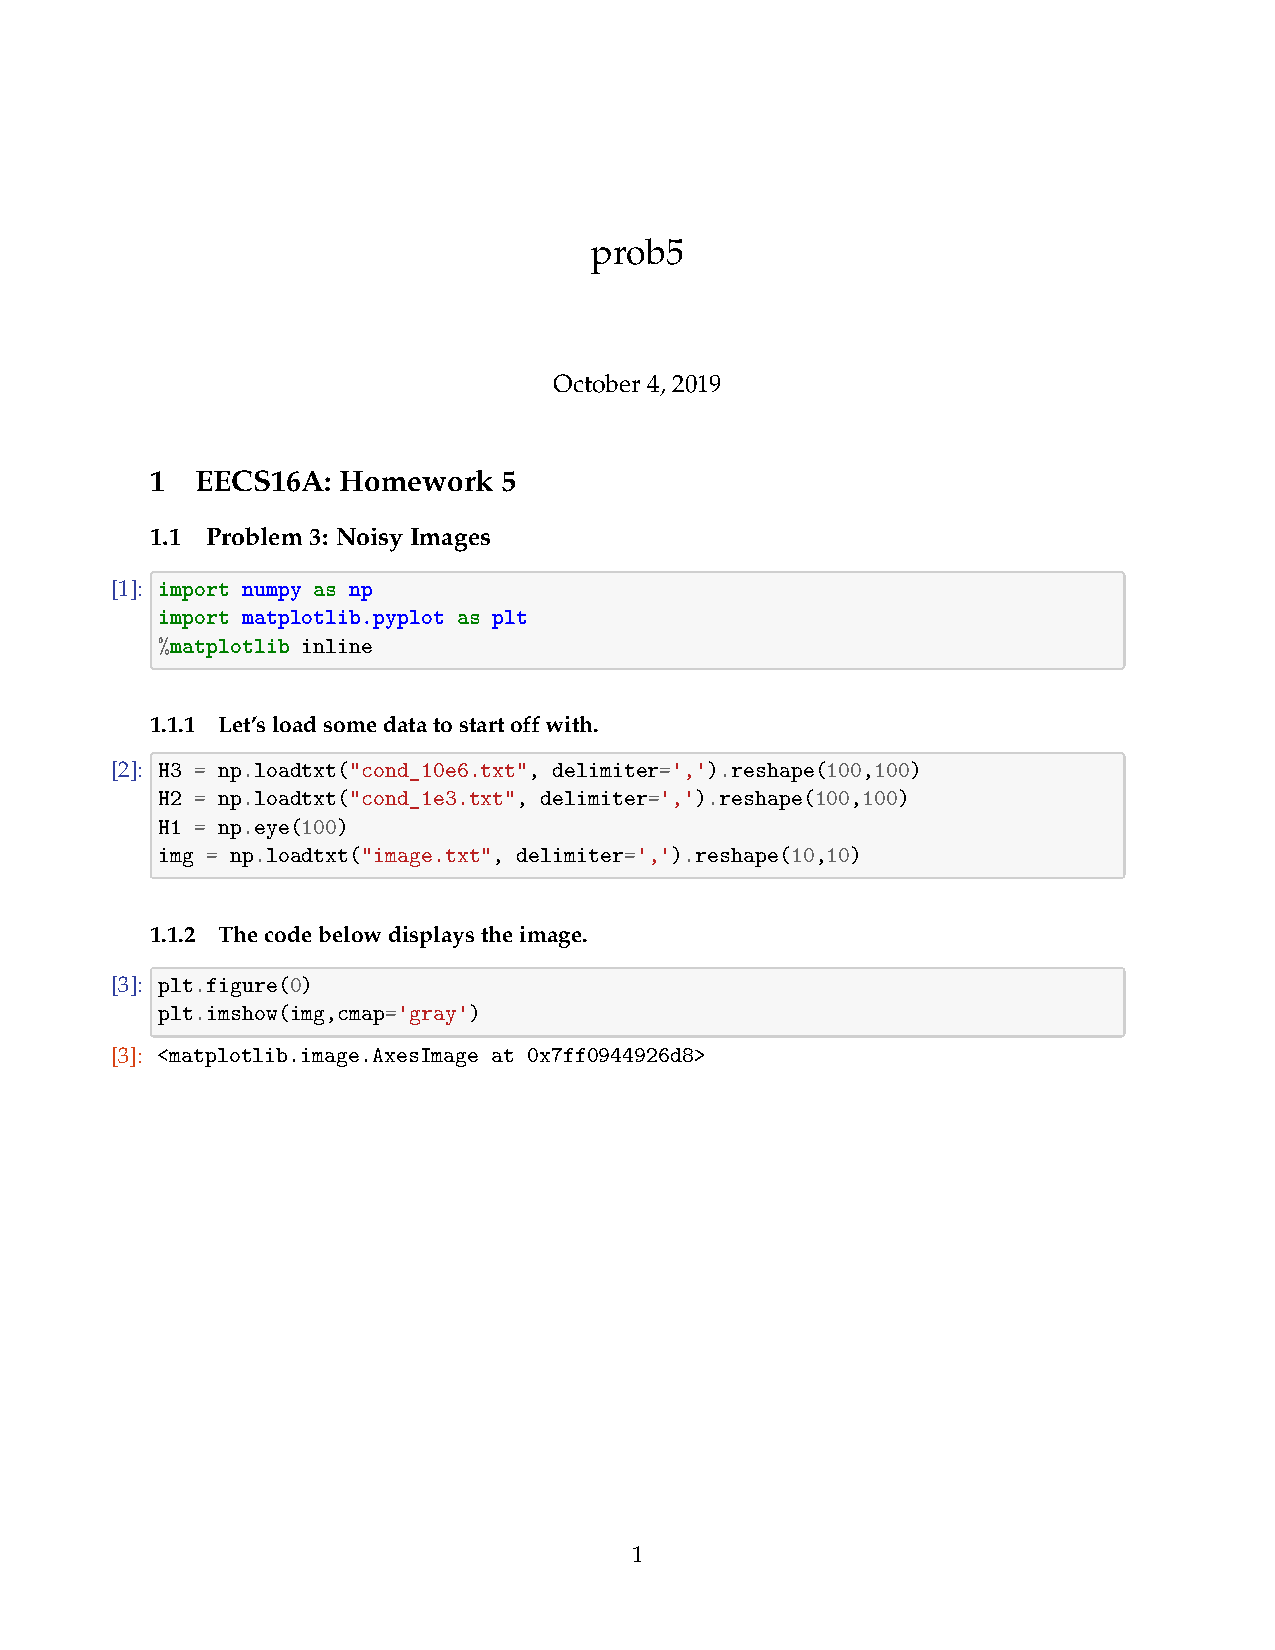
\includepdf[pages=-]{prob5.pdf}

\end{document}